The purpose of our algorithm is to make a three dimensions tracking system, producing position informations 
about a followed target.
The information will be relevant to define parameters 
as: the relative velocity, the factor of approaching and of departure.

The proposed algorithm is shown in Fig. \ref{fig:system};
it begins with a key frame image where a initial target ($ROI$) is determined; 
the system then receives a stream of image frames and the tracking system 
enters into looping follow this target in the next frames.

\begin{figure}[bhp]
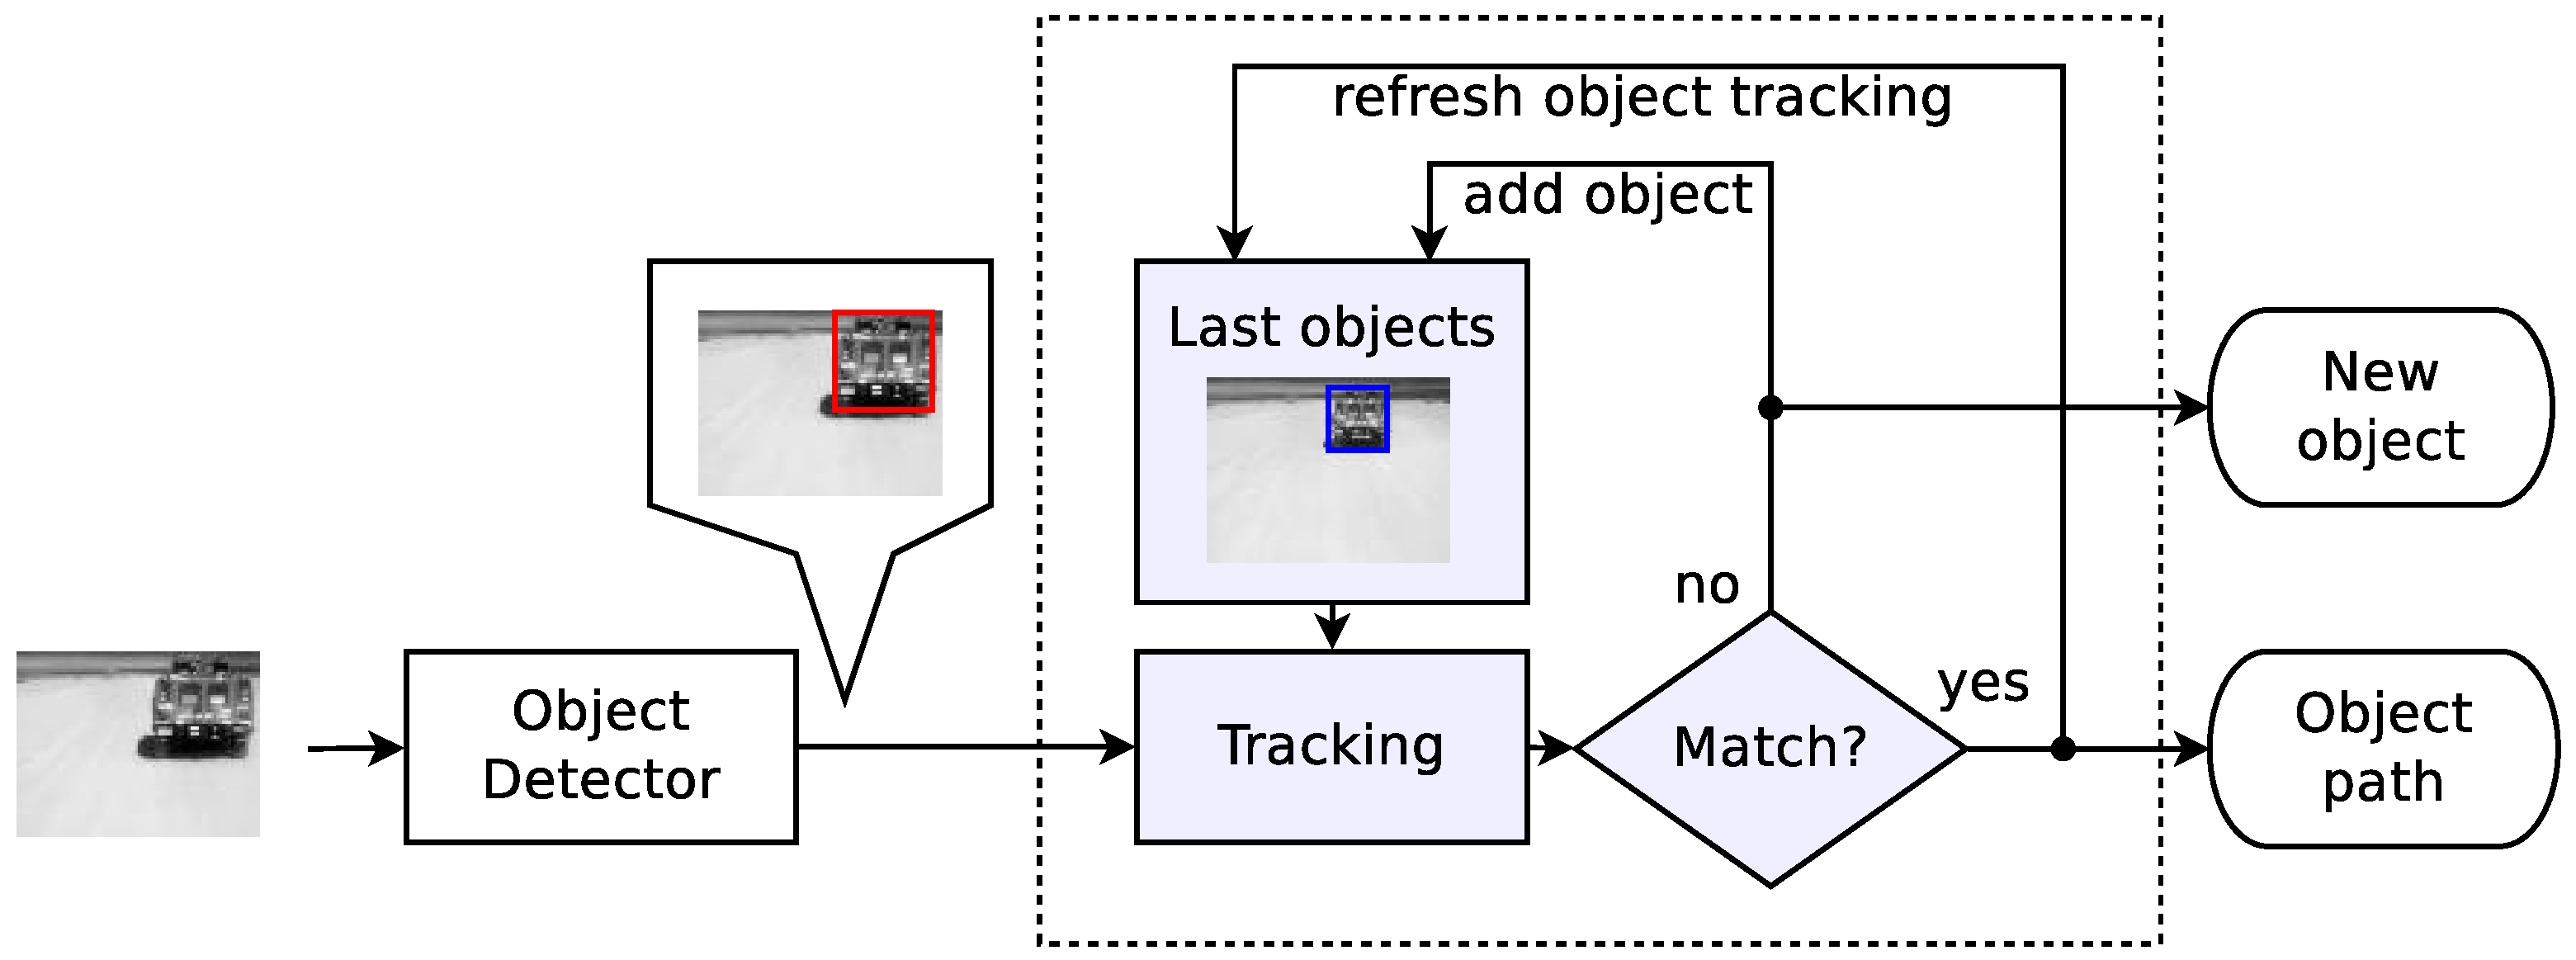
\includegraphics[width=\columnwidth]{images/figure1-diagram1.eps}
\caption{The target is identified from a highest value of correlation (PCC) between a selected ROI and an analysis region in
the $WOS$ of a current frame; the result of this process is a displacement which is  returned as vector field.}
\label{fig:system}
\end{figure}


In a two dimensional analysis, the tracked target given us information about its horizontal 
and vertical position and it is relative to the perpendicular velocity with respect to the observer.
When the target is analyzed in three dimensions, 
the initial $ROI$ has the position $(x=x_0,y=x_0,d=d_0=1)$;
where, $x_0$ and $y_0$ represent a position (horizontal and vertical) in the analyzed image,
and $d_0=1$ represents the initial depth position of target in the $ROI$ (normalized by definition to $1.0$).
Thus, all the results of depth will be relative to this value. In this sense, the relative velocity and 
the factor of approaching or departure can be calculated.

The Algorithm \ref{alg:system} shows a global vision of system described in the 
Fig. \ref{fig:system}, the functions used in the algorithm
will be explicated in the next sections. The algorithm receives as input parameters
A initial $ROI$, your position and a stream of $N$ images; with these data, the
algorithm return a structure called $PATH$ with the position of target in each image frame,
being $PATH\{i\}=(x_i,y_i,d_i)$ the position of analysis region with target in the image $I_i$.

\begin{algorithm}[H]
 \KwData{An initial $ROI$, your position $P_0$ and a stream of images, $I_i$, for $0\leq i < N$. }
 \KwResult{$3D$ target $PATH$ or a target lost message. }
 $i \leftarrow 0$ \;\\
 
\While{$i < N$ }
{
    $\{AR,P,r\} \leftarrow multiscale\_match\_criterion(ROI,P_0,I_i)$\;
    
    $\{ROI,P_0,Found\} \leftarrow renew\_roi\_criteria(ROI,P_0,AR,P,r)$\;
    \eIf{Found}{
      $PATH\{i\}  \leftarrow P$\;
    }{
      break while loop\;
    }
}
\\
\Return PATH \;
\caption{How to get a $3D$ target path.}
\label{alg:system}
\end{algorithm}


%Diagrama1
 %A gente vai explicar o algoritmo como uma caixa fechada , que coisa entra e que coisa sai
 %e os parametros a sintonizar.
 % como usar ele quando implementado, como se fosse uma caixa preta.
